
This application uses the Model-View-Controller MVC pattern to structure the application to create a separation of concern between the main layers of the application. Figure~\ref{fig:impl-layers} shows a high level overview of the architecture and below I discuss the purpose for each.

\begin{figure}[ht]
  \centering
  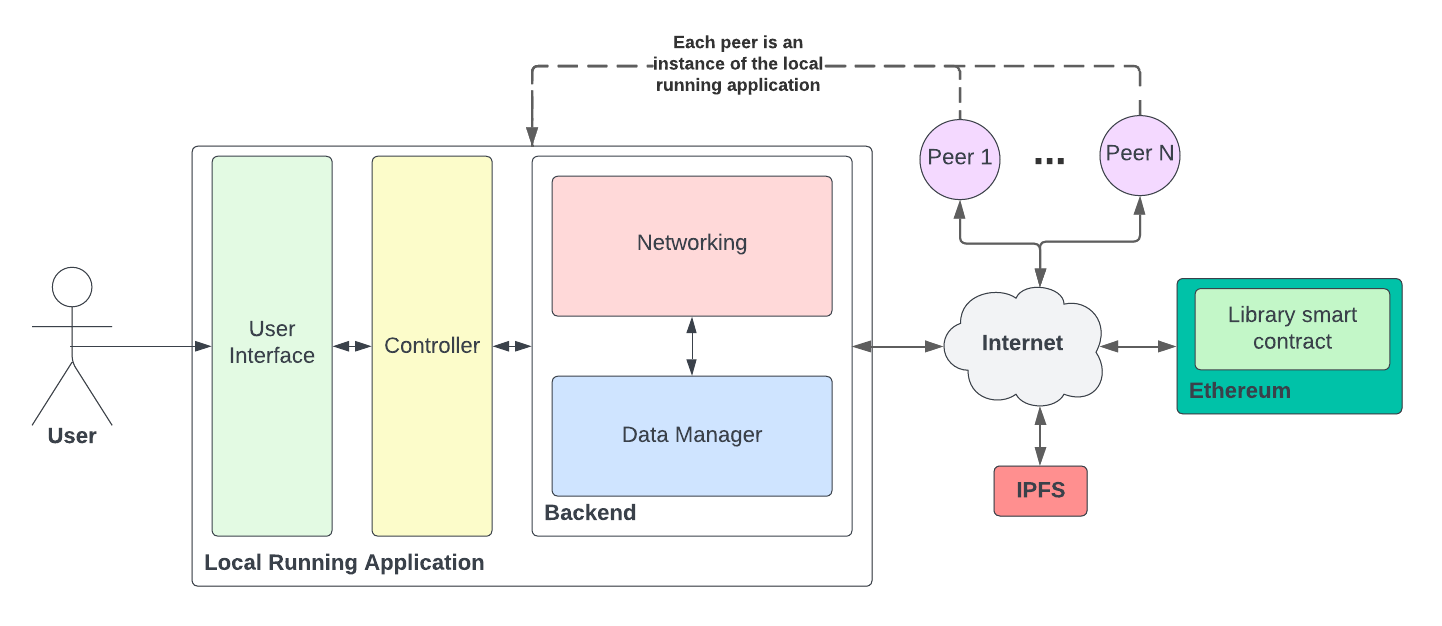
\includegraphics[width=.8\textwidth]{assets/images/diagrams/layers.png}
  \caption{The layers of the application}
  \label{fig:impl-layers}
\end{figure}

% layer entries


\subsection{Persistence}

The Persistence layer shows how the data for the application is divided across several mediums; namely the \textbf{Ethereum Smart Contract}, \textbf{IPFS}, and a \textbf{P2P Network}. Each component stores a different, which is outlined in Section~\ref{subsec:design-data}.
\x
There are several things to note about using Ethereum as platform for selling games:

\begin{itemize}
  \item Ethereum is a less stable currency than most traditional currencies like GBP or USD so games may fluctuate largely in price.
  \item All write functions on the smart contract will incur a gas fee so uploading or updating data will not be free.
  \item Users will have to source Ether from elsewhere before being able to purchase games, which may be intimidating to users not already familiar with the ecosystem.
\end{itemize}

% \subsubsection{Ethereum}\label{subsubsec:impl-eth}

% An Ethereum Smart Contract, written in Solidity \url{https://docs.soliditylang.org/en/v0.8.19/}, will be used to store the set of data about games that is required for the identification of each game. The Smart Contract will also be used to perform the following:
% \x
% The Geth go-ethereum package \url{https://geth.ethereum.org/} will allow us to interact with the ethereum blockchain and Abigen \url{https://docs.avax.network/specs/abigen} will allow us to compile any smart contracts to Go code. This will allow us to interact with our smart contract on ethereum using a set of Go functions. For development, Ganache \url{https://github.com/trufflesuite/ganache} was used to create a local Ethereum instance and Geth was used to connect to an Ethereum test net.


% \subsubsection{IPFS}

% This project will use the IPFS implementation Kubo \url{https://github.com/ipfs/kubo}, due to it being the most widely used implementation of IPFS. We will use the go-ipfs-api library \url{https://github.com/ipfs/go-ipfs-api} to interact with Kubo and upload/download the data specified above.


\subsection*{Backend}\label{subsec:backend}

The Backend can be broken down into two major components:

\begin{itemize}
  \item \textbf{Networking} The creation and maintenance of network connections with other peers over the internet with the purpose of sharing data.
  \item \textbf{Data Manager} the management of local data and the processing of data received and to be uploaded by the Networking component.
\end{itemize}

\subsubsection{Networking}\label{subsubsec:networking}

This component will connect users to the distributed P2P file-sharing network, where it will create and maintain a set of TCP connections with other users \reqref{F-M7} in the network and will communicate by sending structured messages to each other \reqref{F-M8}. Section~\ref{subsubsec:commands} describes these commands in detail.

\paragraph*{Peer Identification}
Peers are identified by their Ethereum addresses, which will allow us to view which games they've purchased and are allowed access to. Upon forming a connection, each peer will request the other return a signature for a generated message, from which we can derive their address and public key.

\paragraph*{Commands}\label{subsubsec:commands}

Structured messages \reqref{F-M8} will typically come as part of a request/response pair involving the sharing of information between peers. Command responses are not awaited to remove unnecessary blocking of the connection channel as a user may be responding to many different requests at once by the same peer. Table~\ref{tab:network-cmds} shows the list of commands used bu the application.

\small
\begin{longtable}{p{.38\textwidth} p{.57\textwidth}}
  \toprule
  \textbf{Message Format} & \textbf{Description}\\
  \midrule\midrule
  LIBRARY
  & Request that a peer sends their library of game.\\
  GAMES;$[hash_1]$;$[hash_2]$;\ldots;
  & The user sends a list of their games as a series of unique root hashes. These root hashes will map to games on the blockchain.\\
  \midrule
  BLOCK;$[gameHash]$;$[blockHash]$;
  & The user will request a block of data off of a peer by sending the root hash of the game and the hash of the block being requested. The response will be a SEND\_BLOCK message \reqref{F-M9} and if it isn't received after a given amount of time then it is resent.\\
  SEND\_BLOCK;$[gameHash]$;\newline $[blockHash]$;$[compressedData]$;
  & The user sends a block of data in response to a BLOCK message \reqref{F-M9}. The data is compressed using the \textit{compress/flate} package to reduce message size \reqref{NF-S1}.\\
  \midrule
  VALIDATE\_REQ;$[message]$
  & The user is requesting for a message to be signed using the receiver's Ethereum private key. This is used to verify the receiver's identity and thus their owned collection of games \reqref{F-S1}.\\
  VALIDATE\_RES;$[signed message]$
  & The user responds to a VALIDATE\_REQ message with a signed version of the received message. From this signature, the receiver can determine the address and public key of the user \reqref{F-S1}.\\
  \midrule
  REQ\_RECEIPT;$[gameHash]$
  & A user will request a RECEIPT message from a peer detailing the data that has been sent by the user for a specific game \reqref{F-S3}.\\
  RECEIPT;$[gameHash]$;$[signature]$\newline ;$[message]$
  & A user will respond to a REQ\_RECEIPT message with a signed message detailing all of the blocks that the requester has sent to the user from a given game. This will allow for users to prove their contributions to the game developer who could then reward them \reqref{F-S3}.\\
  \midrule
  REQ\_PEERS
  & A user requests the list of peers which the receiver peer is connected to. This will be sent immediately after a peer's identity is validated and will help increase the connectivity in the network \reqref{F-S4}.\\
  PEERS;$[p_1 hostname]:[p_1 port]$;\ldots
  & A user will send a list of their active peers. This will be limited to those peers which they have connected to and thus know the hostname and port of their server \reqref{F-S4}.\\
  SERVER;$[hostname]:[port]$
  & When we form a connection with a peer we send them the address of our server that peers use to connect to us. This allows that peer to share our address through the PEER command so we are more easily discoverable.\\
  \midrule
  ERROR;$[message]$
  & An error message that can be used to prompt a peer to resend a message.\\
  \bottomrule\bottomrule
  \caption{The set of structured messages sent between peers}
  \label{tab:network-cmds}
\end{longtable}
\normalsize
\subsubsection{Data Manager}\label{subsubsec:data-manager}

This component is responsible for interacting with local storage and managing the user's collection of owned and installed games.
It will interact directly with Ethereum to discover, purchase \reqref{F-M5}, and upload \reqref{F-M1} \reqref{F-M2} games and use IPFS to upload and distribute game assets \reqref{F-C2} and hash trees \reqref{F-M12}.

\paragraph*{Download Order} Each download will have a downloader thread that selects the order at which blocks are to be fetched. Using the hash tree, it will queue whole files at a time and to verify the whole file once all blocks have been fetched.





\subsubsection*{Optimisations}

\paragraph*{Worker Pools}
Tasks are queued down a FIFO channel and each one is collected by a single worker thread who will perform a specific task based upon what data was sent. This allowed us to have many worker threads listening on the same channel who will complete tasks in parallel to largely increase the performance of the application.

\vspace{2mm}\noindent
Some of the areas this pattern was used include:

\begin{itemize}
  \item Sharding files to create a hash tree,
  \item To locate and request blocks from many downloads at once, and
  \item To insert received data and free up the thread listening on a connection,
\end{itemize}

\paragraph*{Ignore File} A standard implementation of a .ignore file was included to indicate to the hash tree algorithm which files/folders to ignore. This is useful to ignore temporary or non-static files, which contents will vary by user and thus won't need to be distributed.

\subsection*{Frontend \& Controller}

\subsubsection{Frontend}\label{subsubsec:frontend}

This application will have a GUI \reqref{F-S2} \reqref{NF-S2} where users can interact with the platform. Having a GUI is essential to making the platform as easy to use as possible so that it is accessible to new users. At minimum it will need to include the following pages:

\begin{itemize}
  \item \textbf{Library} The user's collection of owned games, where they can view details for each game as well as manage their download status.
  \item \textbf{Store} Where user's can find and purchase new games that have been uploaded by other users.
  \item \textbf{Upload} Where users can fill in details about their new or updated game and have it be uploaded to the network.
  \item \textbf{Downloads} Where user's can track all of their ongoing downloads and see their progress.
  \item \textbf{Peers} Where users can manage their list of connected peers. Here a user can form new connections, break existing ones and request specific data from their peers.
  \item \textbf{Help} A help page to describe the application and all of its functionality \reqref{NF-C1}
\end{itemize}

\newparagraph
To satisfy \reqref{NF-M3}, a developer must always be displayed with both their chosen name and their Ethereum address. A developer should publically provide their Ethereum address to ensure their users can identify it.

\subsubsection{Controller}

The Controller will be represented as a set of interface functions that allow the backend and frontend code to communicate. This can be done to trigger actions such as starting a game download or to fetch data like the list of a user's owned games.

\section{Controller}

The Wails package will generate controller functions that can be called by the frontend to trigger events or fetch data from the backend. It also includes the ability for the backend to trigger runtime events that tell the frontend to perform a specific action. This allowed me to easily create a reactive frontend.

